\section*{CHƯƠNG 5 - KẾT QUẢ DEMO}
\addcontentsline{toc}{section}{\numberline{}CHƯƠNG 5 -  KẾT QUẢ DEMO}
\setcounter{section}{5}
\setcounter{subsection}{0}
\setcounter{figure}{0}
\setcounter{table}{0}

%-------------Phần trình bày nội dung chương 5

\subsection{ Tự động cấu hình hóa VLAN:}
\_Kết nối và cấu hình VLAN cho Switch1:

    \begin{figure}[H]
        \centering
        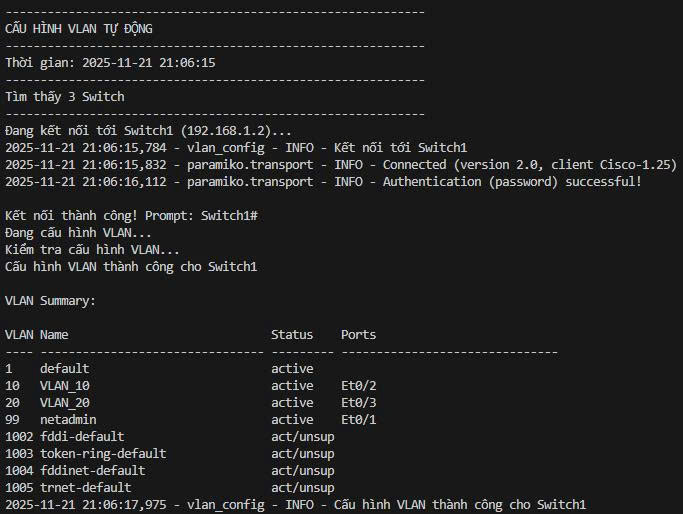
\includegraphics[width=0.7\textwidth]{image/vlan_1.jpg}
        \caption{Cấu hình VLAN cho Switch1}
    \end{figure} % Bắt buộc phải có lệnh này

\_Kết nối và cấu hình VLAN cho Switch2:

     \begin{figure}[H]
        \centering
        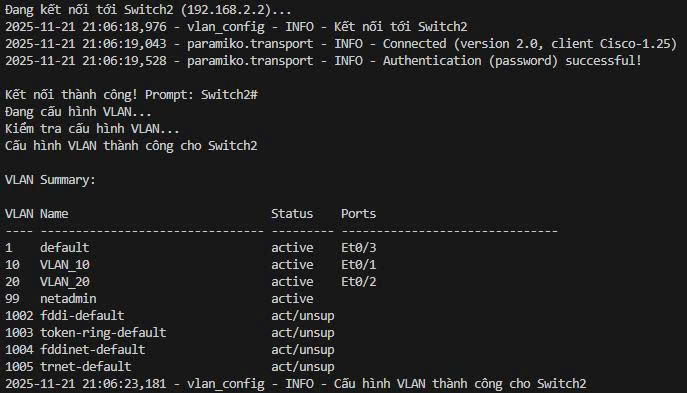
\includegraphics[width=0.7\textwidth]{image/vlan_2.jpg}
        \caption{Cấu hình VLAN cho Switch2}
    \end{figure} % Bắt buộc phải có lệnh này

\_Kết nối và cấu hình VLAN cho Switch3:

    \begin{figure}[H]
        \centering
        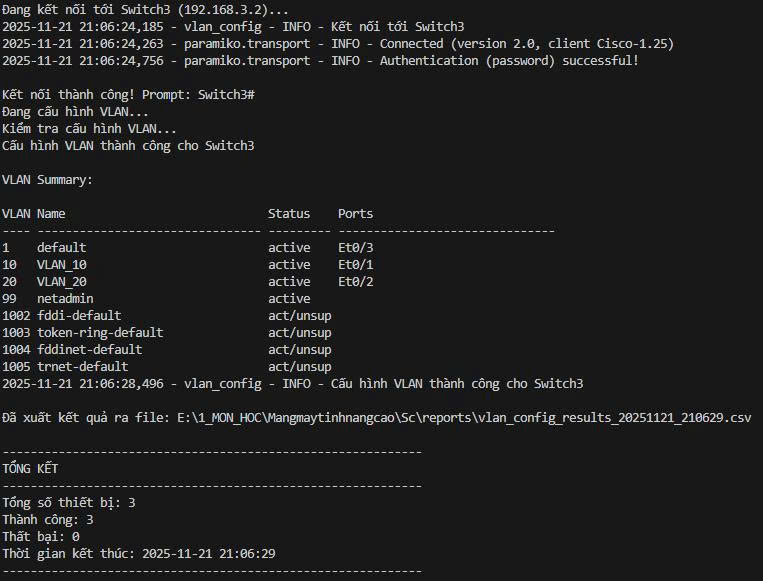
\includegraphics[width=0.7\textwidth]{image/vlan_3.jpg}
        \caption{Cấu hình VLAN cho Switch3}
    \end{figure} % Bắt buộc phải có lệnh này

\subsection{Tự động hóa cấu hình IP:}

\_Kết nối và cấu hình IP cho Router1:

    \begin{figure}[H]
        \centering
        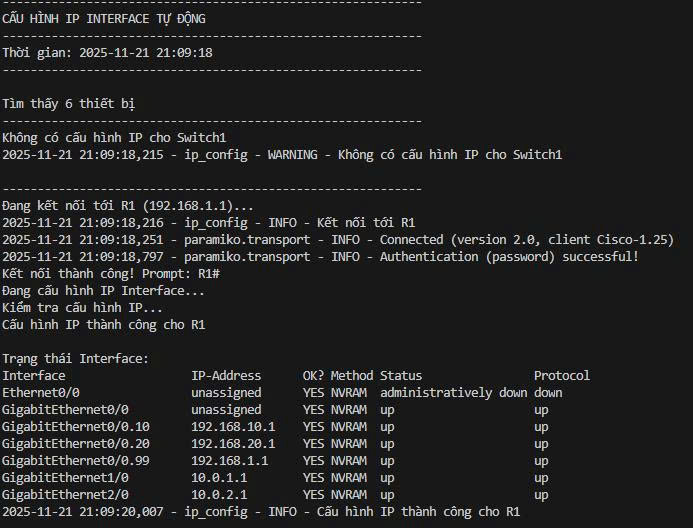
\includegraphics[width=0.7\textwidth]{image/IP_1.jpg}
        \caption{Cấu hình IP cho Router1}
    \end{figure} % Bắt buộc phải có lệnh này

\_Kết nối và cấu hình IP cho Router2:

    \begin{figure}[H]
        \centering
        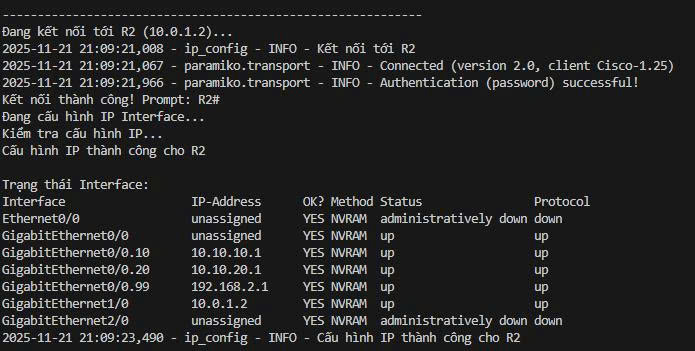
\includegraphics[width=0.7\textwidth]{image/IP_2.jpg}
        \caption{Cấu hình IP cho Router2}
    \end{figure} % Bắt buộc phải có lệnh này

\_Kết nối và cấu hình IP cho Router3:

    \begin{figure}[H]
        \centering
        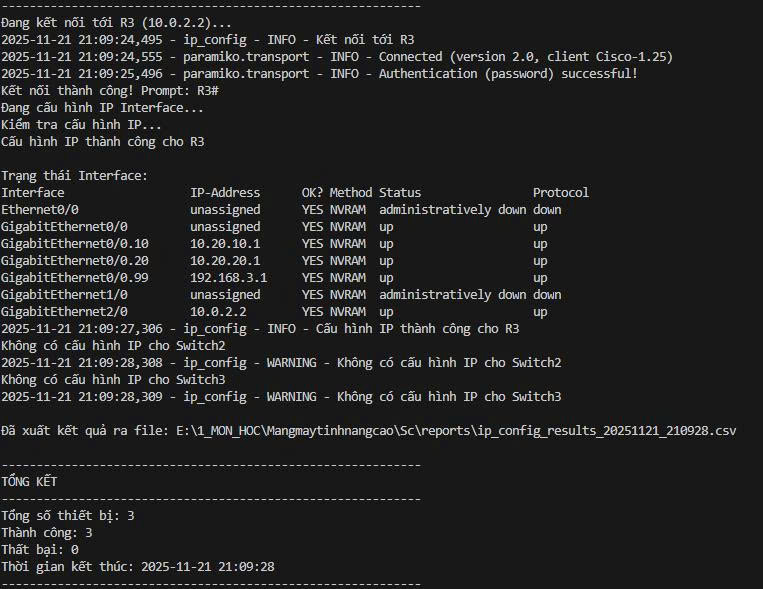
\includegraphics[width=0.7\textwidth]{image/IP_3.jpg}
        \caption{Cấu hình IP cho Router3}
    \end{figure} % Bắt buộc phải có lệnh này

\subsection{Tự động hóa cấu hình OSPF:}

\_Kết nối và cấu hình OSPF cho Router1:

    \begin{figure}[H]
        \centering
        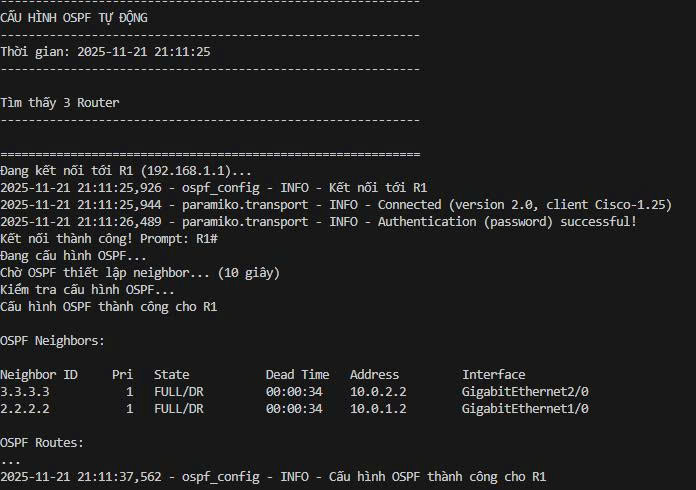
\includegraphics[width=0.7\textwidth]{image/OSPF_1.jpg}
        \caption{Cấu hình OSPF cho Router1}
    \end{figure} % Bắt buộc phải có lệnh này

\_Kết nối và cấu hình OSPF cho Router2:

    \begin{figure}[H]
        \centering
        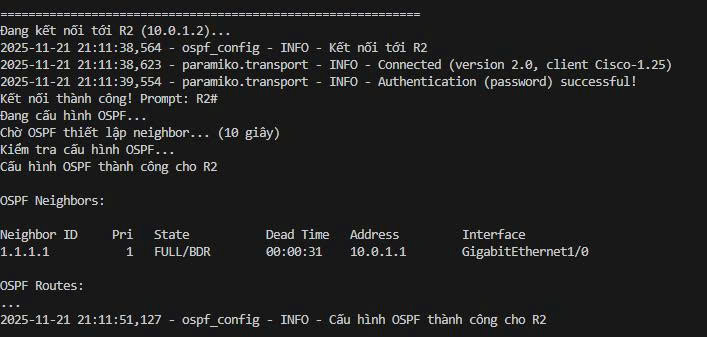
\includegraphics[width=0.7\textwidth]{image/OSPF_2.jpg}
        \caption{Cấu hình OSPF cho Router2}
    \end{figure} % Bắt buộc phải có lệnh này

\_Kết nối và cấu hình OSPF cho Router3:

    \begin{figure}[H]
        \centering
        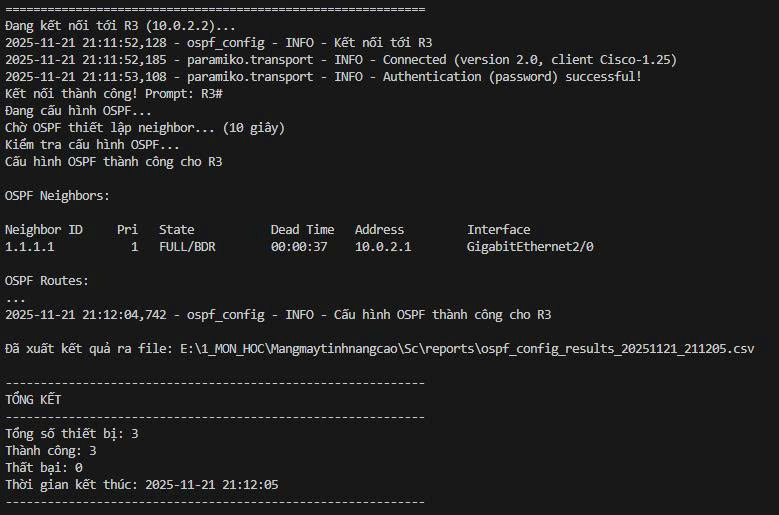
\includegraphics[width=0.7\textwidth]{image/OSPF_3.jpg}
        \caption{Cấu hình OSPF cho Router3}
    \end{figure} % Bắt buộc phải có lệnh này

\subsection{Tự động hóa cấu hình STATIC:}

\_Kết nối và cấu hình STATIC\_ROUTE cho Router1:

    \begin{figure}[H]
        \centering
        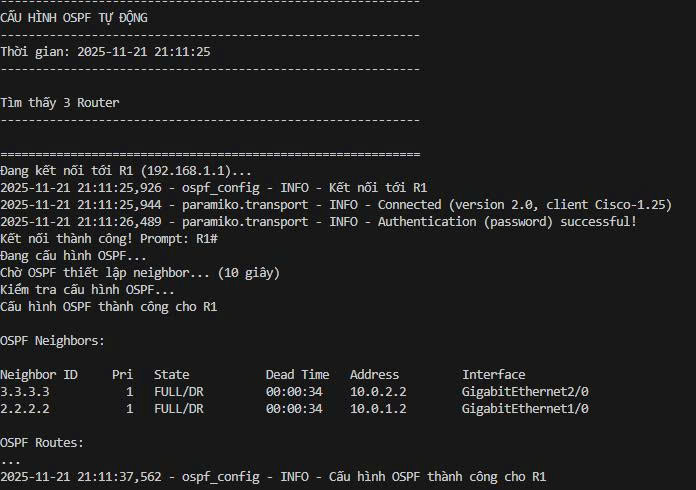
\includegraphics[width=0.7\textwidth]{image/OSPF_1.jpg}
        \caption{Cấu hình STATIC\_ROUTE cho Router1}
    \end{figure} % Bắt buộc phải có lệnh này

\_Kết nối và cấu hình STATIC\_ROUTE cho Router2:

    \begin{figure}[H]
        \centering
        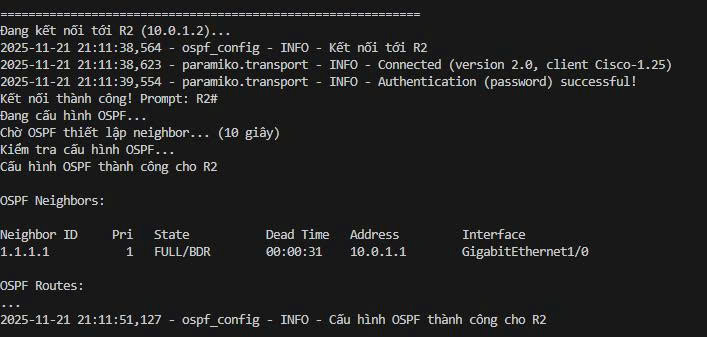
\includegraphics[width=0.7\textwidth]{image/OSPF_2.jpg}
        \caption{Cấu hình STATIC\_ROUTE cho Router2}
    \end{figure} % Bắt buộc phải có lệnh này

\_Kết nối và cấu hình STATIC\_ROUTE cho Router3:

    \begin{figure}[H]
        \centering
        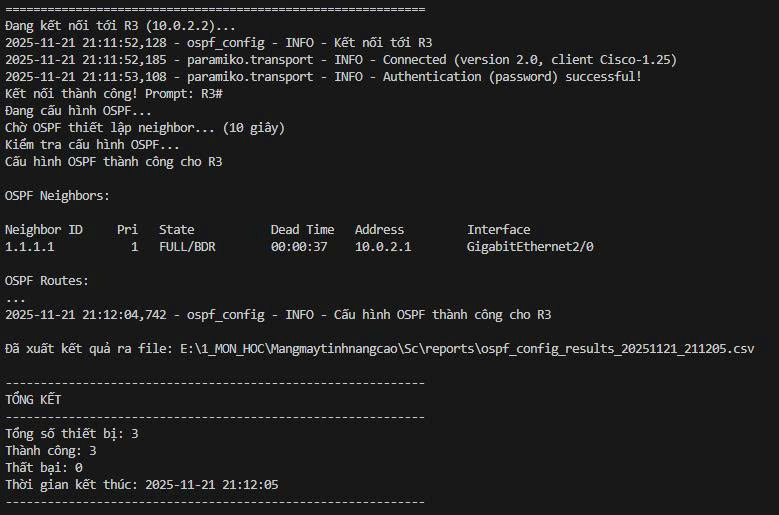
\includegraphics[width=0.7\textwidth]{image/OSPF_3.jpg}
        \caption{Cấu hình STATIC\_ROUTE cho Router3}
    \end{figure} % Bắt buộc phải có lệnh này

\subsection{Cấu hình cho back\_up và restore:}

    \begin{figure}[H]
        \centering
        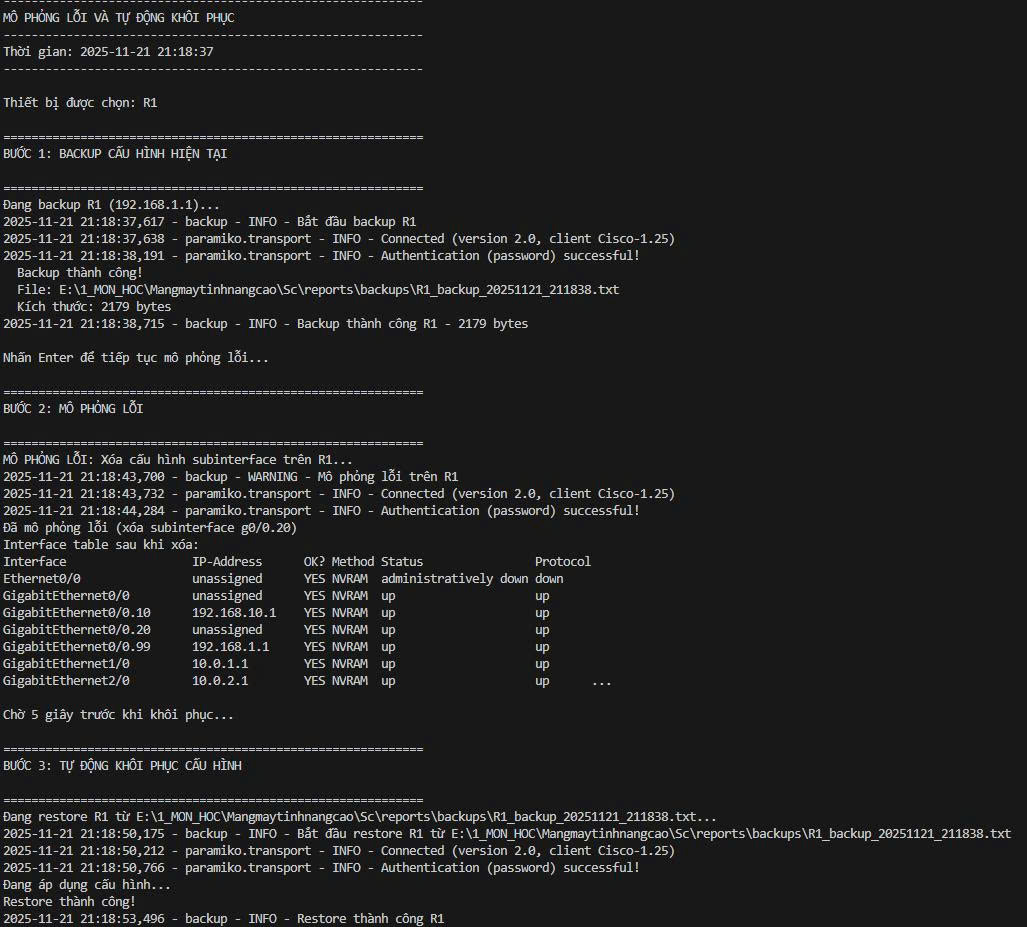
\includegraphics[width=0.7\textwidth]{image/back_up&rstore.jpg}
        \caption{Cấu hình back\_up\&restore}
    \end{figure} % Bắt buộc phải có lệnh này

\subsection{Tự động cấu hình giám sát:}
\_Kiểm tra kết nối thiết bị:

    \begin{figure}[H]
        \centering
        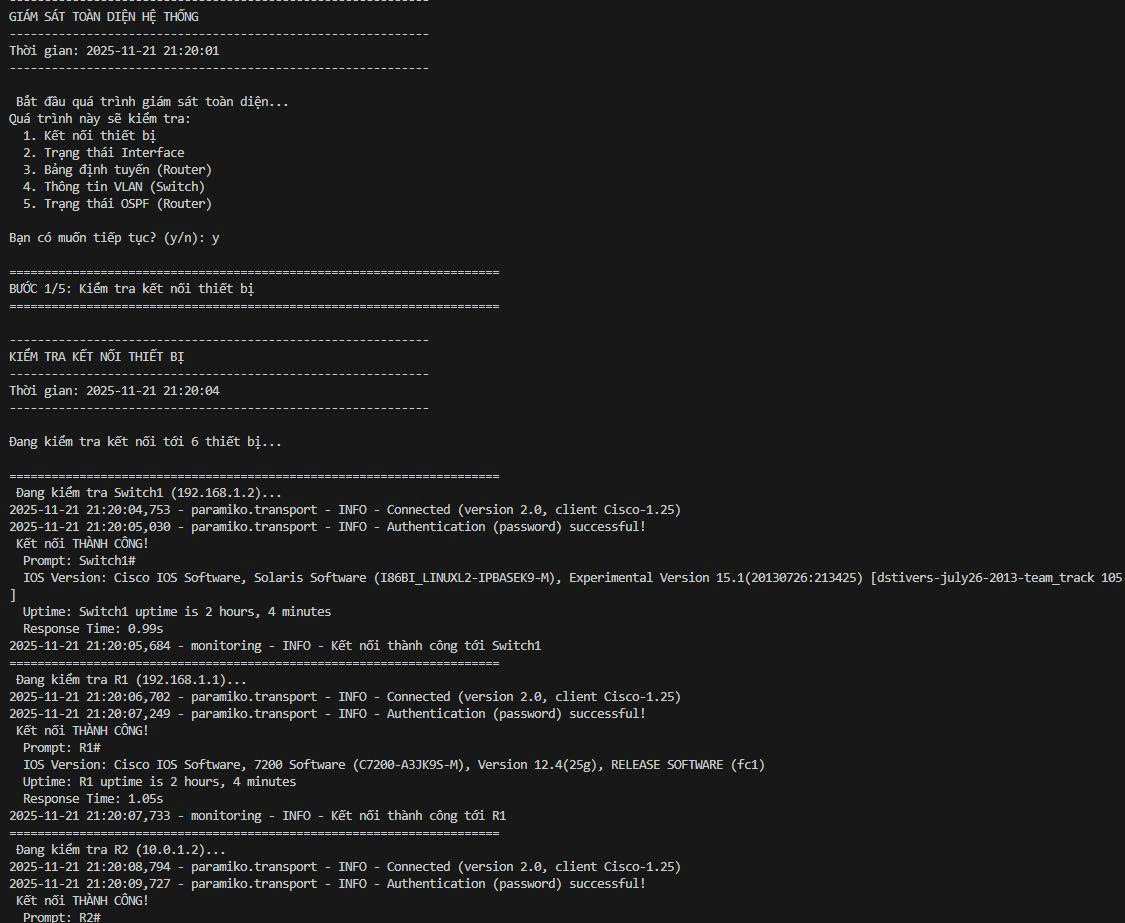
\includegraphics[width=0.7\textwidth]{image/mn_1.jpg}
        \caption{Thực hiện kiểm tra kết nối}
    \end{figure} % Bắt buộc phải có lệnh này

    \begin{figure}[H]
        \centering
        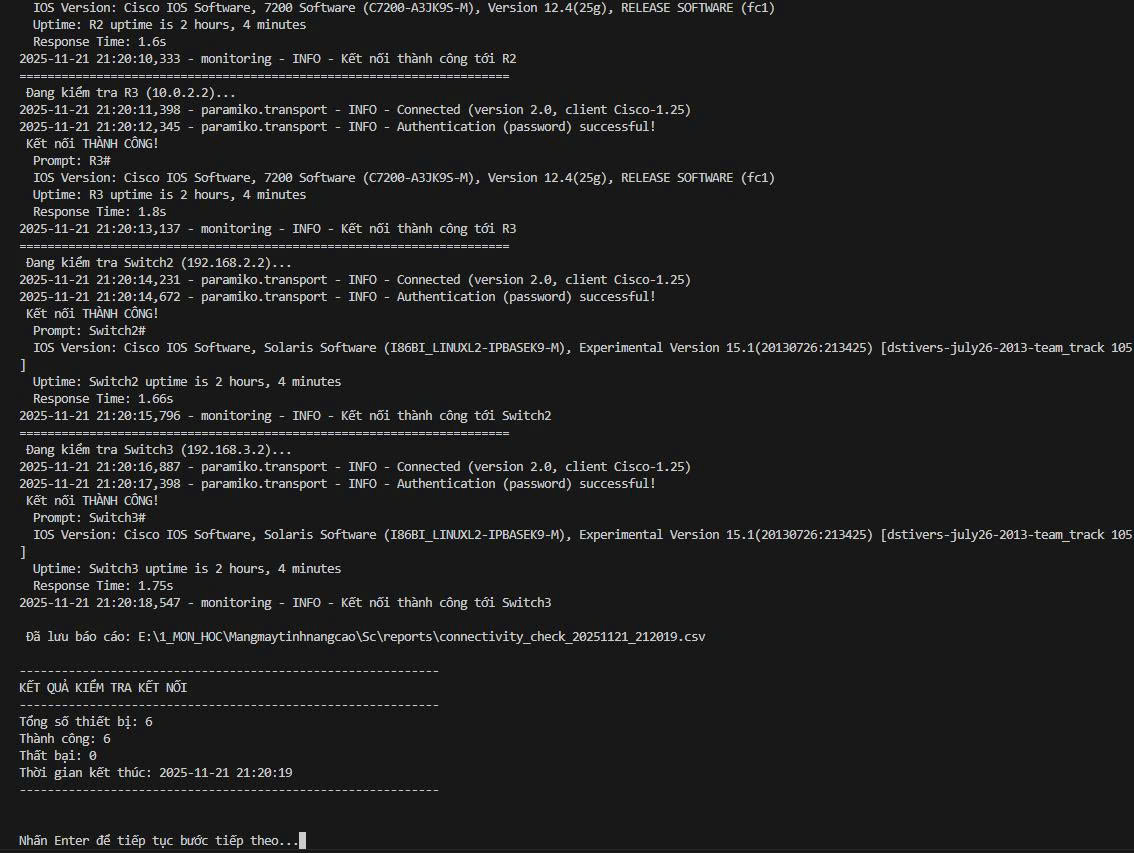
\includegraphics[width=0.7\textwidth]{image/mn_2.jpg}
        \caption{Thực hiện kiểm tra kết nối}
    \end{figure} % Bắt buộc phải có lệnh này

\_Kiểm tra trạng thái interface:

    \begin{figure}[H]
        \centering
        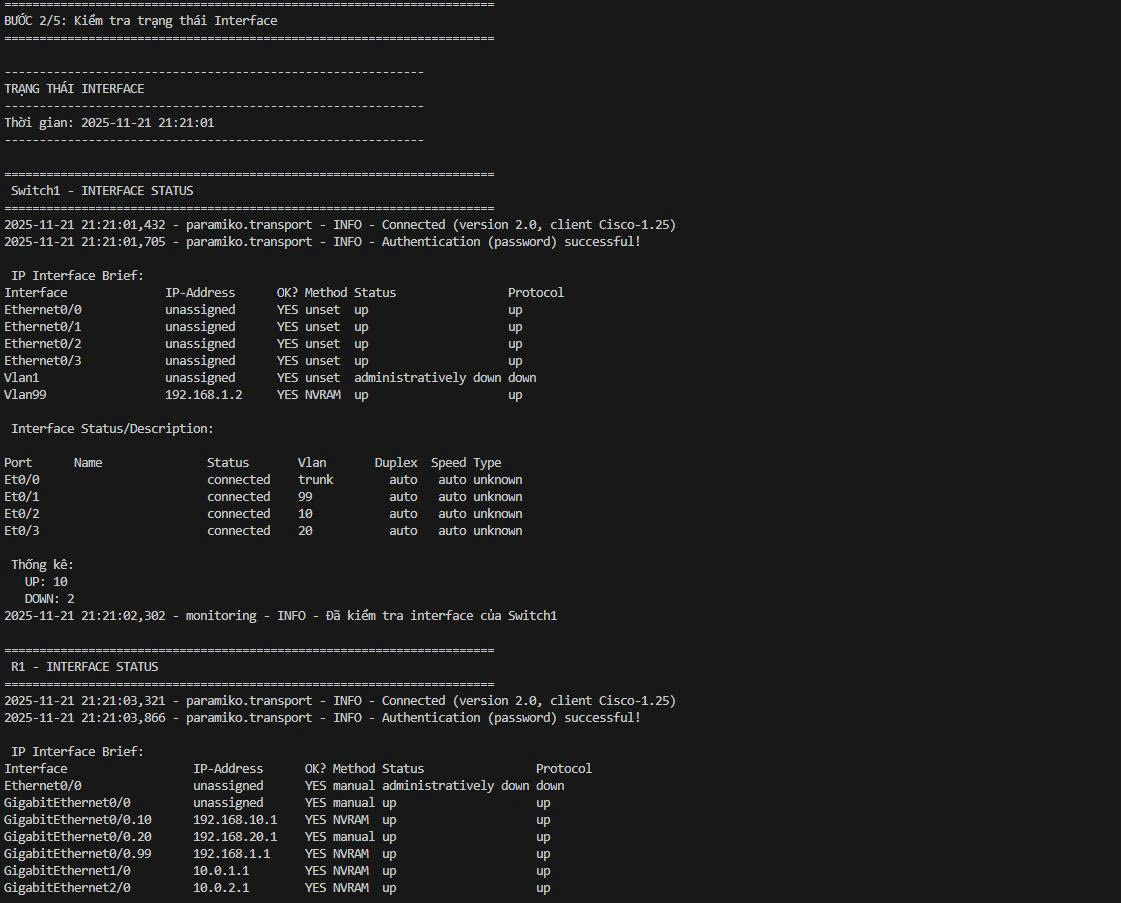
\includegraphics[width=0.7\textwidth]{image/mn_3.jpg}
        \caption{Kiểm tra trạng thái interface}
    \end{figure} % Bắt buộc phải có lệnh này

    \begin{figure}[H]
        \centering
        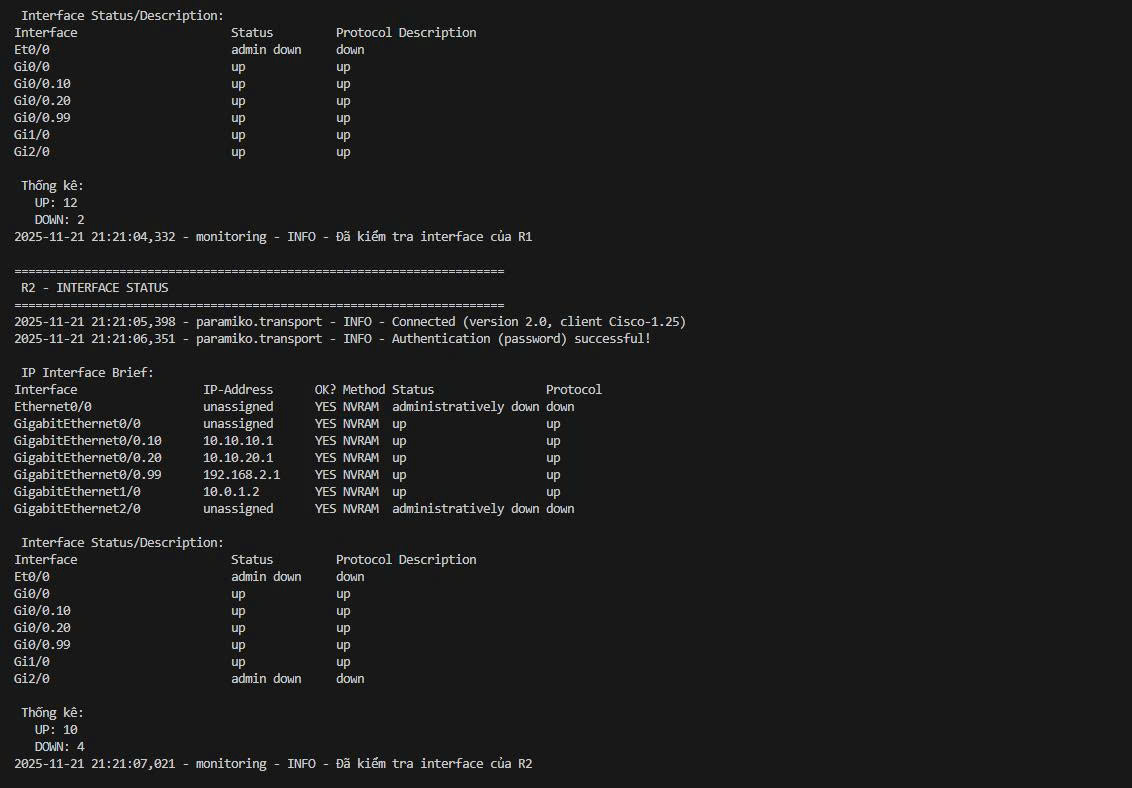
\includegraphics[width=0.7\textwidth]{image/mn_4.jpg}
        \caption{Kiểm tra trạng thái interface}
    \end{figure} % Bắt buộc phải có lệnh này

    \begin{figure}[H]
        \centering
        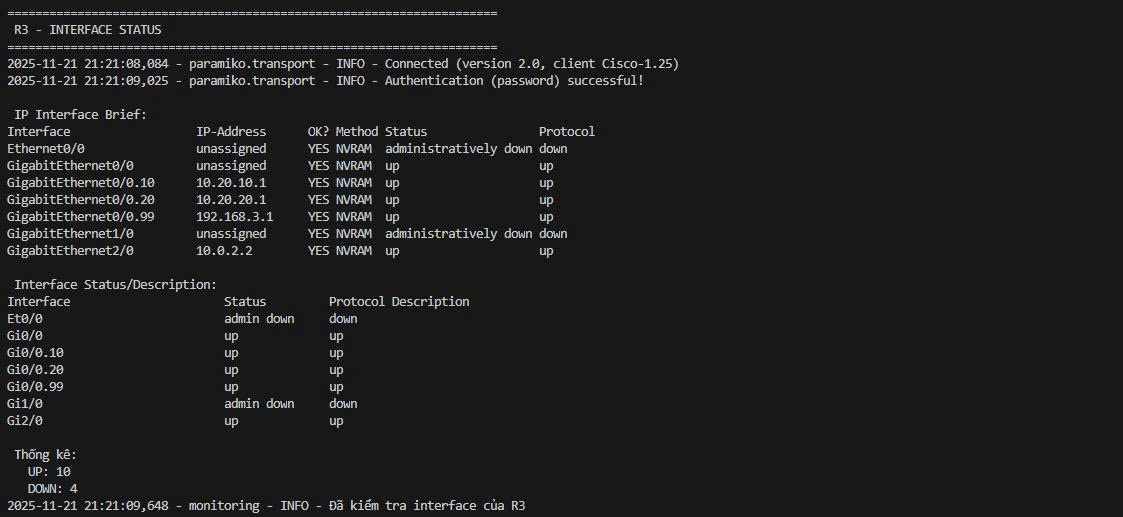
\includegraphics[width=0.7\textwidth]{image/mn_5.jpg}
        \caption{Kiểm tra trạng thái interface}
    \end{figure} % Bắt buộc phải có lệnh này

    
    \begin{figure}[H]
        \centering
        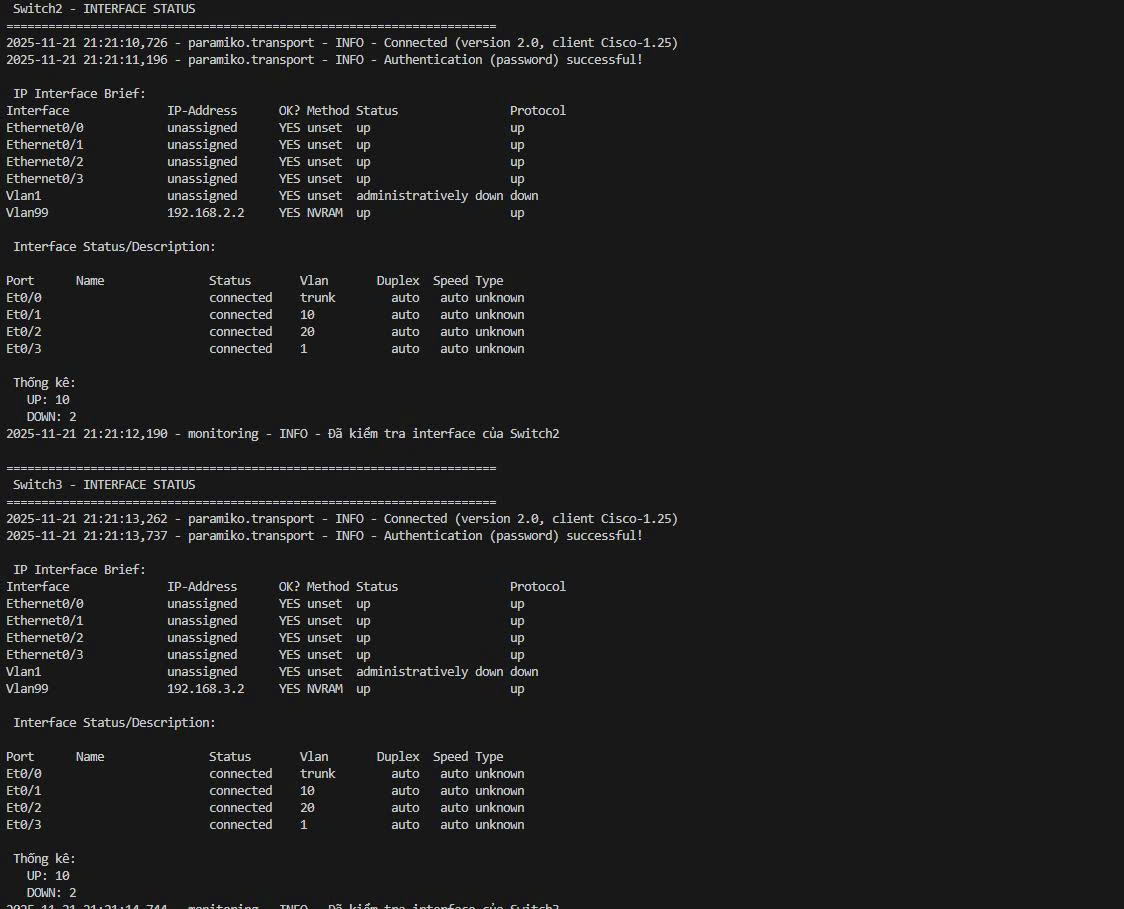
\includegraphics[width=0.7\textwidth]{image/mn_6.jpg}
        \caption{Kiểm tra trạng thái interface}
    \end{figure} % Bắt buộc phải có lệnh này

\_Kiểm tra định tuyến:

    \begin{figure}[H]
        \centering
        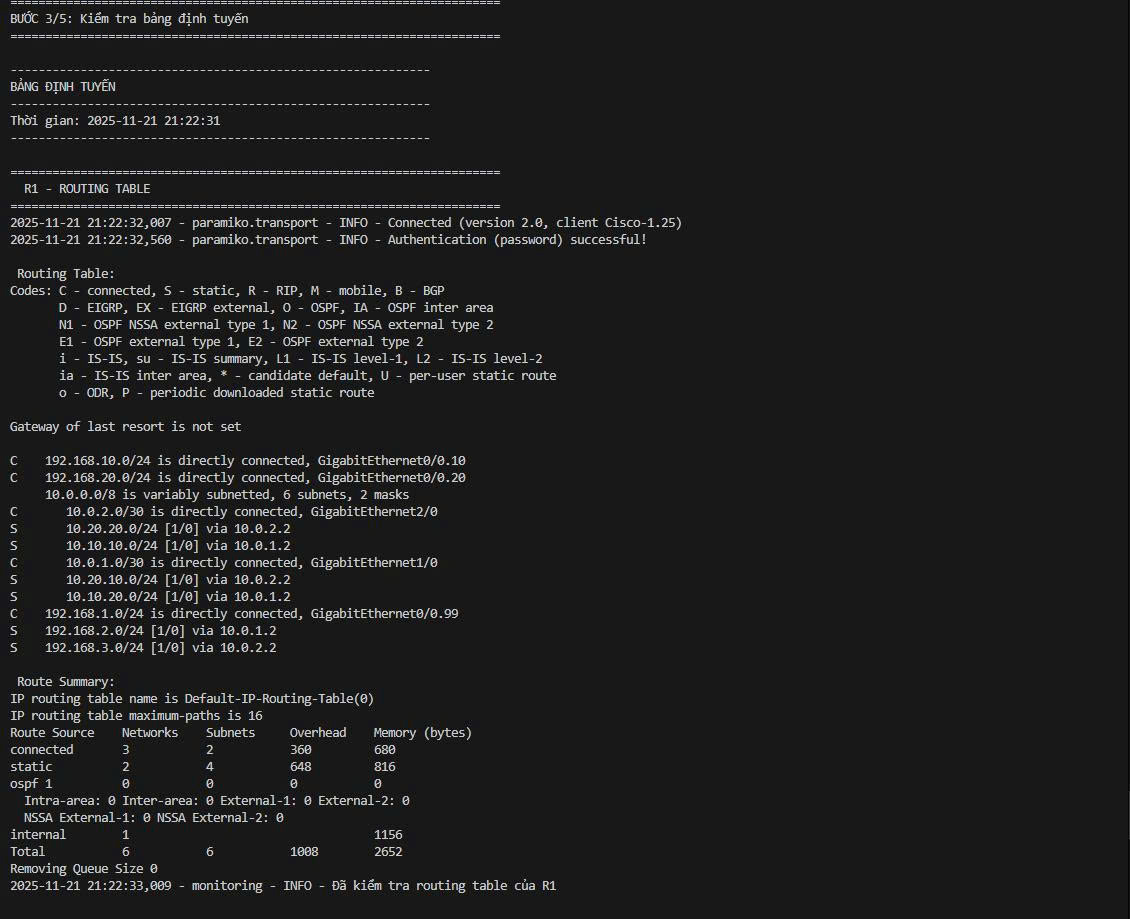
\includegraphics[width=0.7\textwidth]{image/mn_7.jpg}
        \caption{Kiểm tra định tuyến}
    \end{figure} % Bắt buộc phải có lệnh này

    \begin{figure}[H]
        \centering
        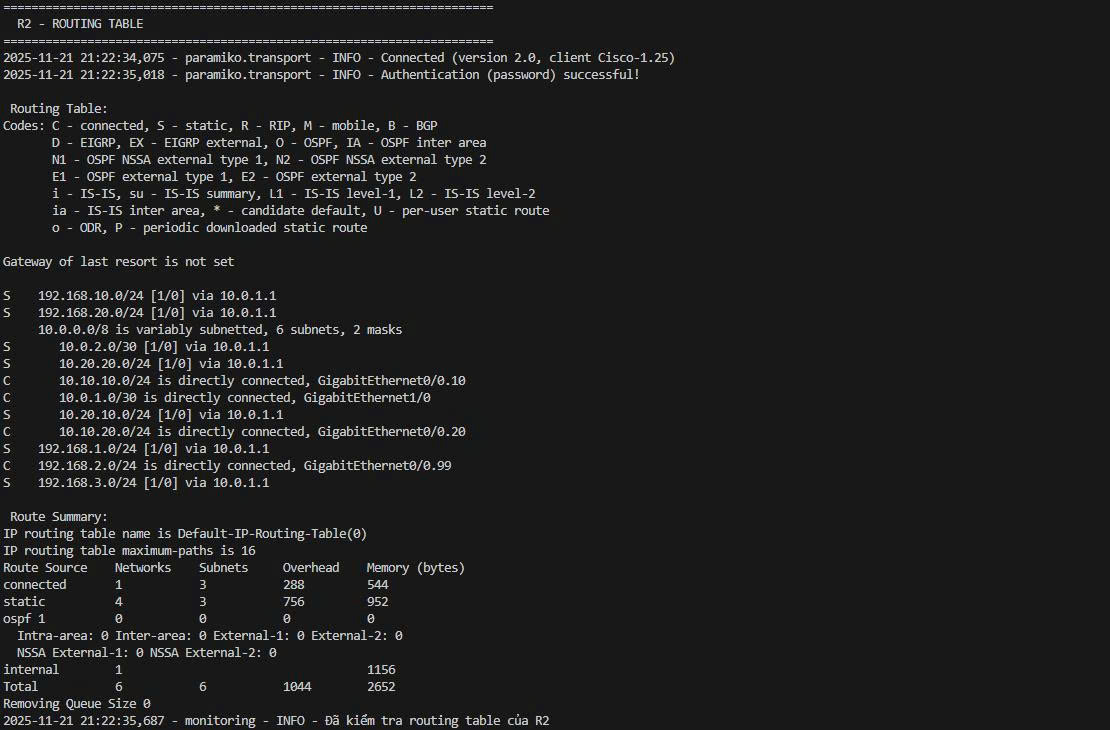
\includegraphics[width=0.7\textwidth]{image/mn_8.jpg}
        \caption{Kiểm tra định tuyến}
    \end{figure} % Bắt buộc phải có lệnh này

    \begin{figure}[H]
        \centering
        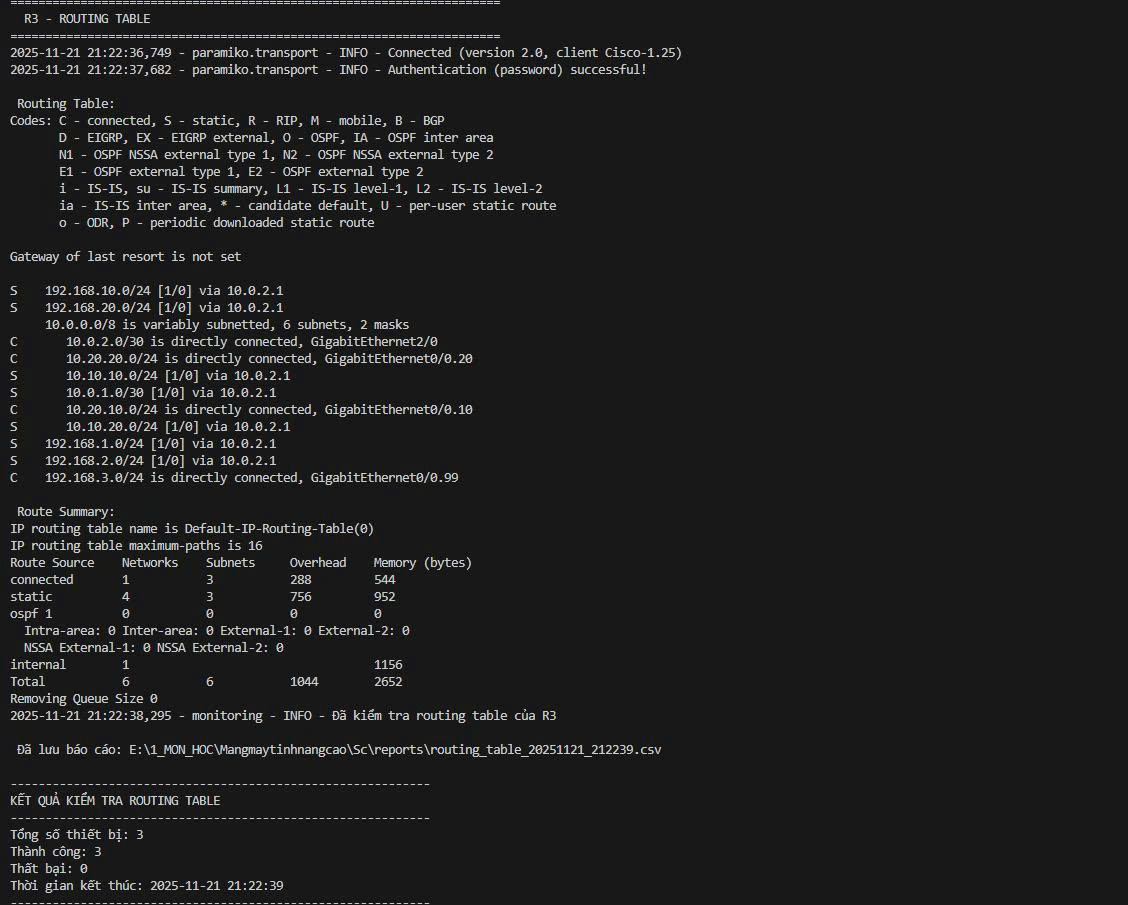
\includegraphics[width=0.7\textwidth]{image/mn_9.jpg}
        \caption{Kiểm tra định tuyến}
    \end{figure} % Bắt buộc phải có lệnh này

\_Kiểm tra cấu hình VLAN:

    \begin{figure}[H]
        \centering
        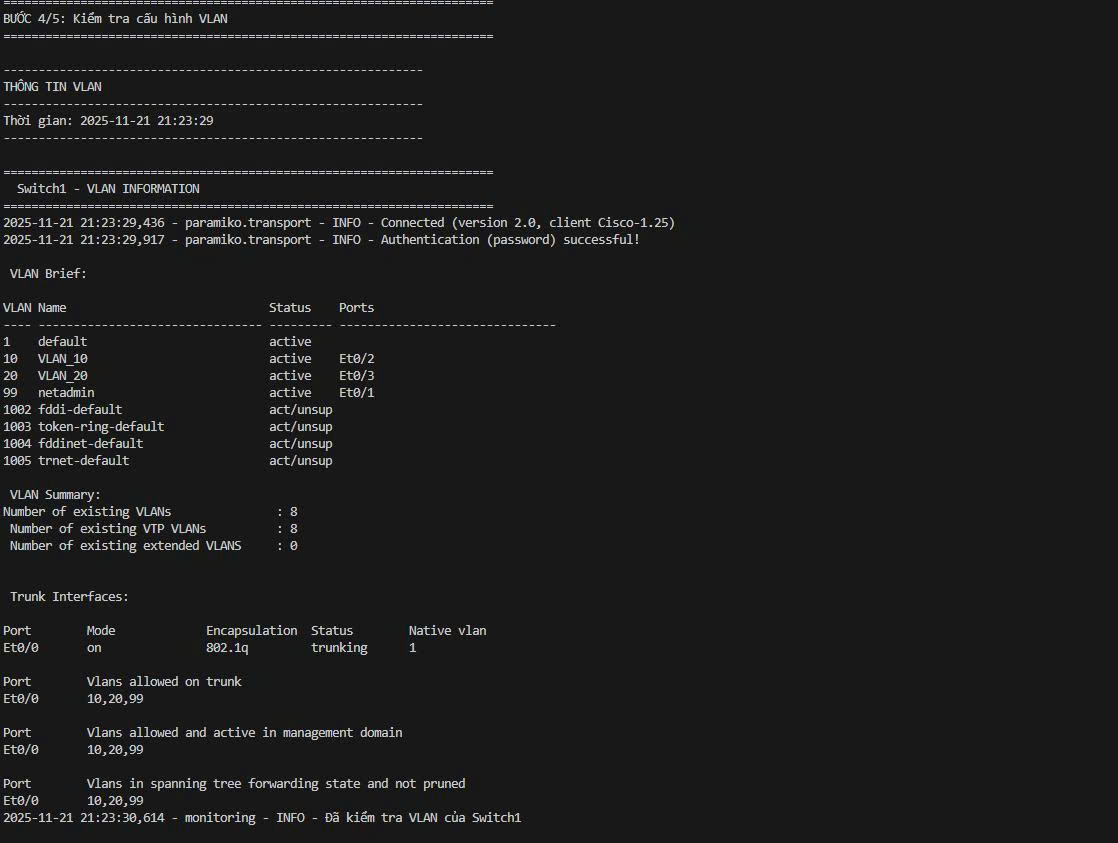
\includegraphics[width=0.7\textwidth]{image/mn_10.jpg}
        \caption{Kiểm tra cấu hình VLAN}
    \end{figure} % Bắt buộc phải có lệnh này

    \begin{figure}[H]
        \centering
        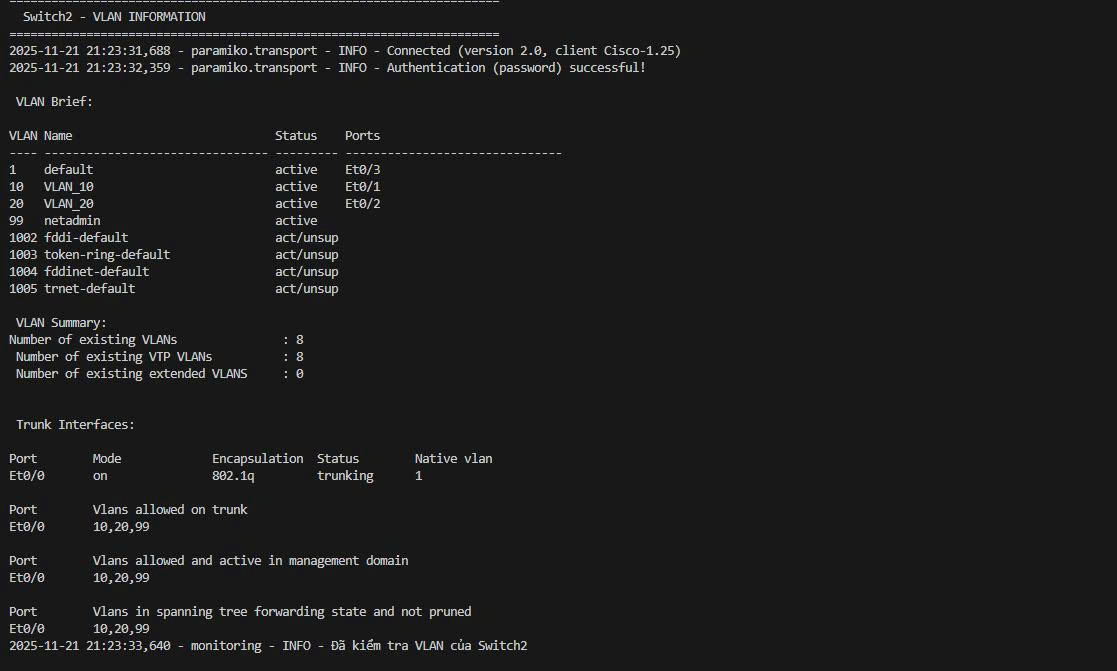
\includegraphics[width=0.7\textwidth]{image/mn_11.jpg}
        \caption{Kiểm tra cấu hình VLAN}
    \end{figure} % Bắt buộc phải có lệnh này

    \begin{figure}[H]
        \centering
        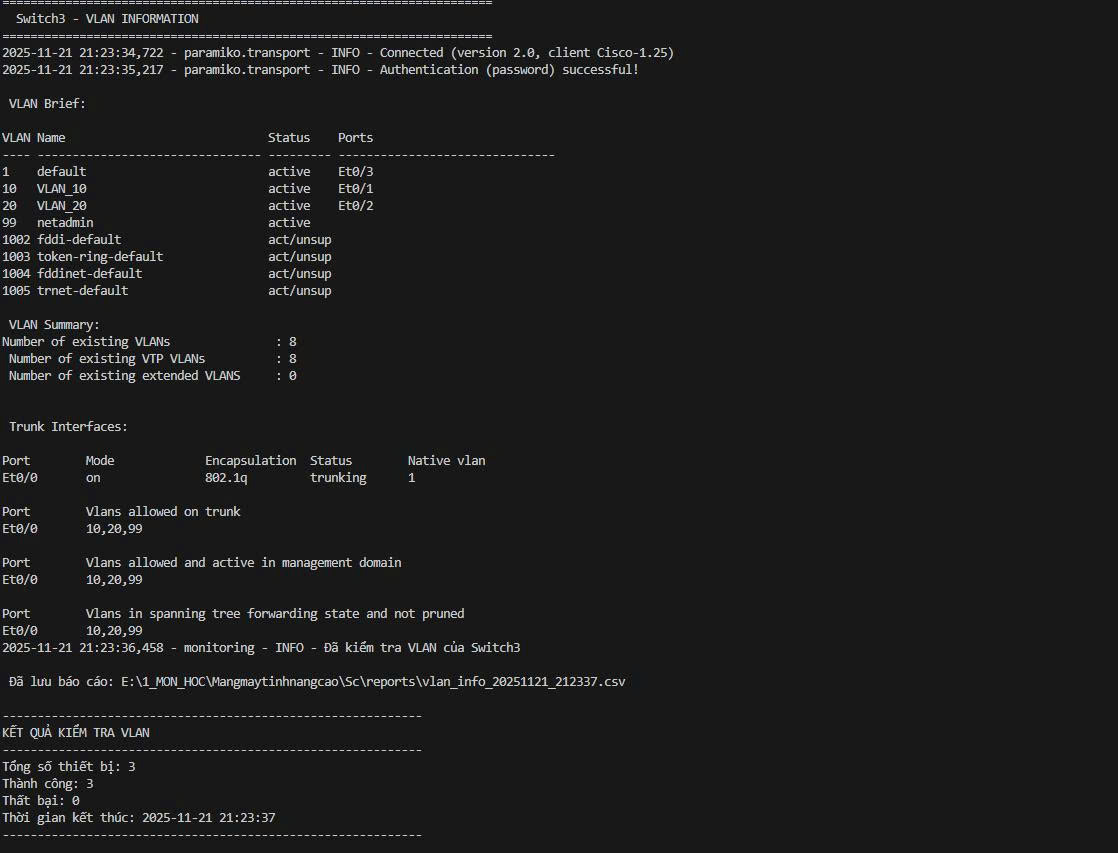
\includegraphics[width=0.7\textwidth]{image/mn_12.jpg}
        \caption{Kiểm tra cấu hình VLAN}
    \end{figure} % Bắt buộc phải có lệnh này

\_Kiểm tra trạng thái OSPF:

    \begin{figure}[H]
        \centering
        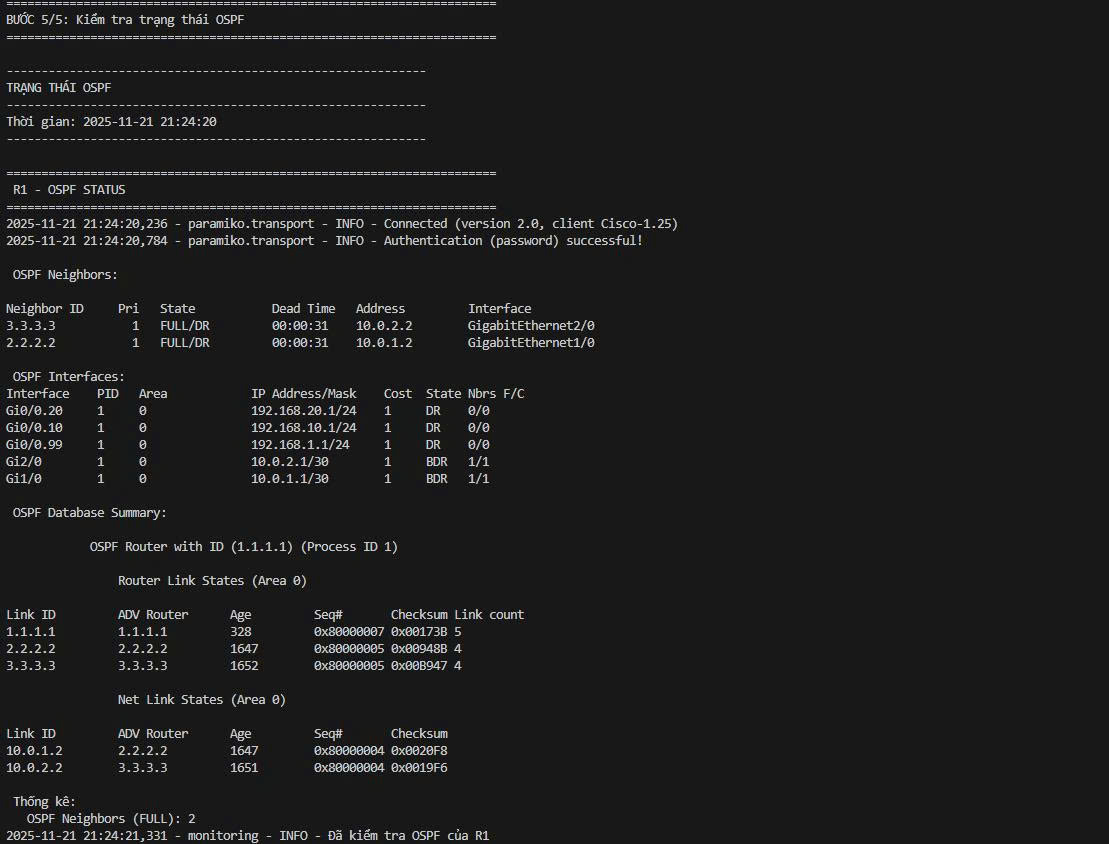
\includegraphics[width=0.7\textwidth]{image/mn_13.jpg}
        \caption{Kiểm tra trạng thái OSPF}
    \end{figure} % Bắt buộc phải có lệnh này

    \begin{figure}[H]
        \centering
        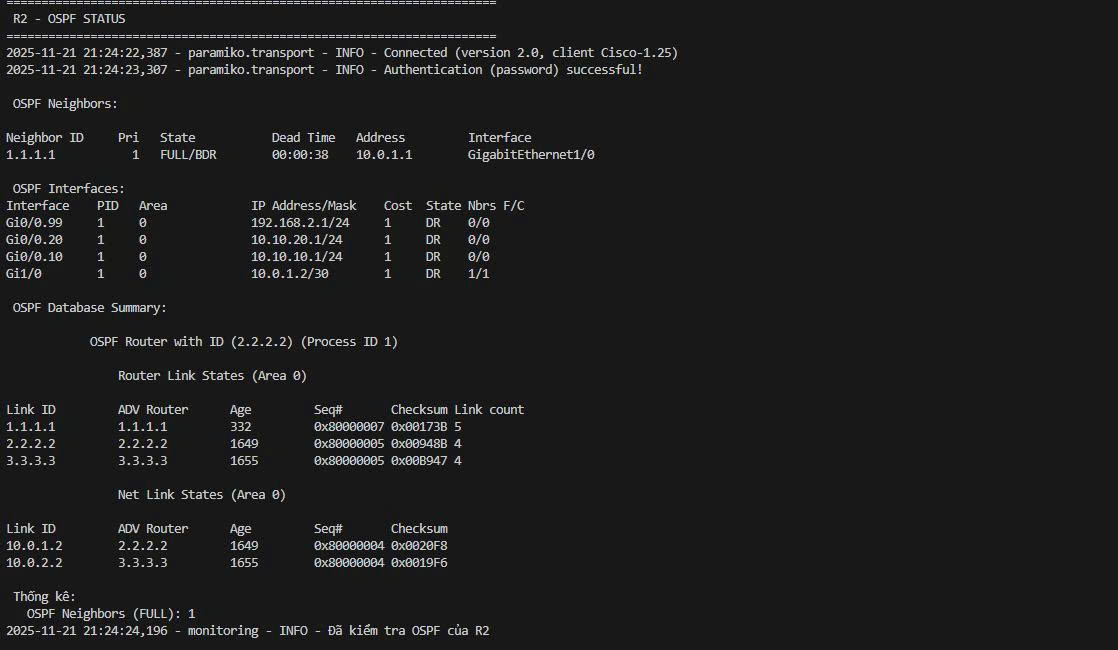
\includegraphics[width=0.7\textwidth]{image/mn_14.jpg}
        \caption{Kiểm tra trạng thái OSPF}
    \end{figure} % Bắt buộc phải có lệnh này

    \begin{figure}[H]
        \centering
        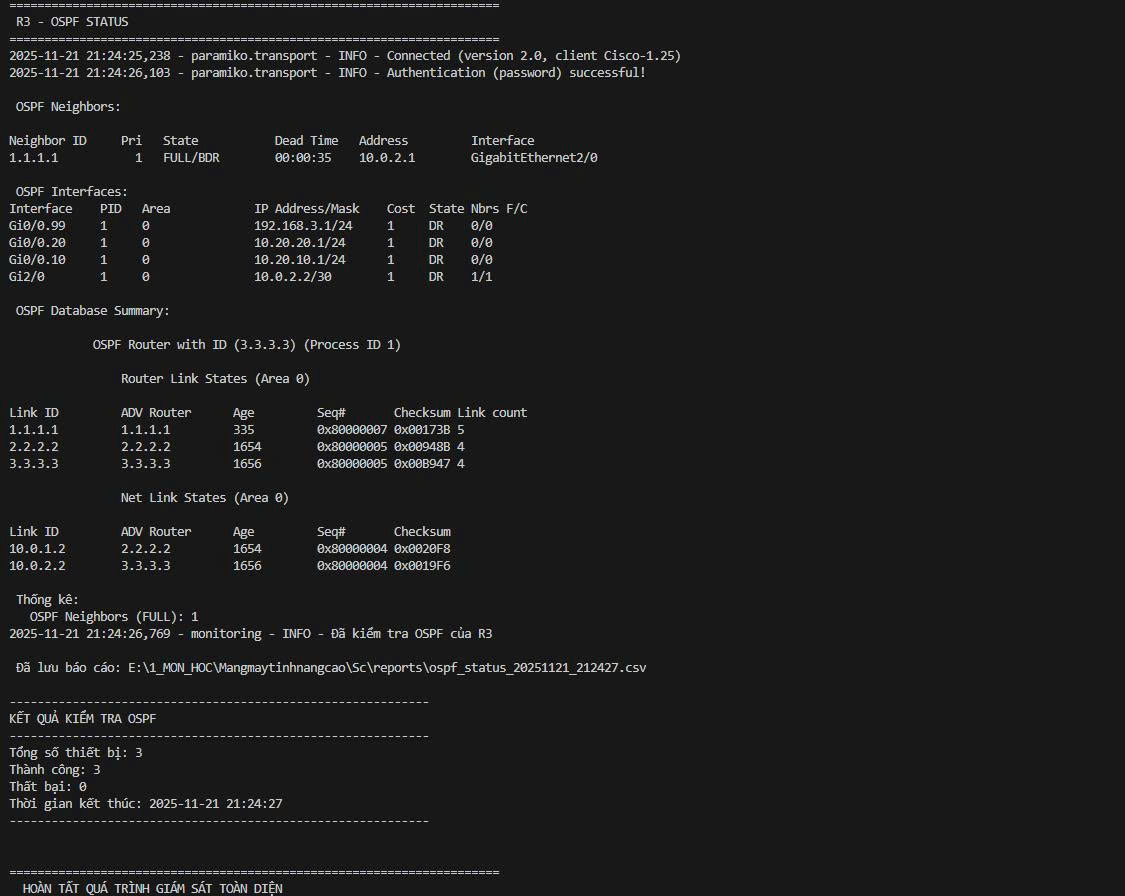
\includegraphics[width=0.7\textwidth]{image/mn_15.jpg}
        \caption{Kiểm tra trạng thái OSPF}
    \end{figure} % Bắt buộc phải có lệnh này